\subsection{Network experiments}
The network experiments have been performed to analyze the dA network and establish global characteristics of the network, but also to find interesting sub-networks of artists and artworks which are of particular interest to investigate.

The dA network consists of 13 million registered artists, and therefore doing a full analysis of the the whole network was not possible within the time-scope of the project. Therefore a network of the dA watchers functionality\footnote{A watcher is someone who indicates he likes an artist and would like to receive updates when that artist produces new artwork.} was extracted for all except casual artists (distinguished with a \textit{tilde} ($\sim$)). This network formed the basis of our network experiments.

From this large network of around 100000 professional artists three core-networks were extracted using the \textit{FindCore} algorithm, described in Algorithm \ref{alg:findcore}. The three cores correspond to three types of the $degree(j)$ function in that algorithm, namely: in-degree, out-degree and in+out-degree. This has resulted in a core of artists that are \textit{power-watchers}, a core with \textit{popular-watched} artists and last a mix of both.

The results of the network experiments are presented in Table \ref{tab:netstatistics}, Table \ref{tab:netcooccurrences} as well as Figure \ref{fig:results_core}.  For all networks, statistics were extracted. Unfortunately for the large professional artists network, statistics such as the characteristic path length were not within the time-scope of this project.

\begin{table}[htb]
    \centering
    \begin{tabular}
        { | l | r | r | r | r | r | r |} 
        \hline
        Network &  prof.  & watchers & watched & mixed\\
	            &  artists & core & core & core \\
        \hline
	no. nodes $(n)$& 103663 & 1701 & 1471 & 1099 \\
	no. links & 4483023 & 139285 & 127837  & 166244 \\
	avg. degree $(k)$& 43.25 & 81.88 & 86.90 & 151.27 \\
	findcore $\max x$ & - & 43 & 44 & 185\\
	$L_G$ & - & 2.15 & 2.27 & 2.14 \\
	$L_{random}$ & - & 1.69 & 1.63 & 1.40 \\
	$C_G$ & - & 0.20 & 0.22 & 0.20 \\
	$C_{random}$ & - & 0.048 & 0.059 & 0.140 \\
	\hline
    \end{tabular}
    \caption{Network statistics}
    \label{tab:netstatistics}
\end{table}
\begin{table}[htb]
    \centering
    \begin{tabular}
        { | l | c | c | c |} 
        \hline
        core Network & watchers & watched & mixed\\
        co-occurrences  &   core & core & core \\
        \hline
        watchers core & 1701 &541& 54\\
        watched core & 541 &1471& 286\\
        mixed core  &54 &286 &1099\\
	\hline
    \end{tabular}
    \caption{Core network co-occurrences, there are 14 artists which are in all 3 core networks}
    \label{tab:netcooccurrences}
\end{table}

\begin{figure*}[htb]
  \centering
  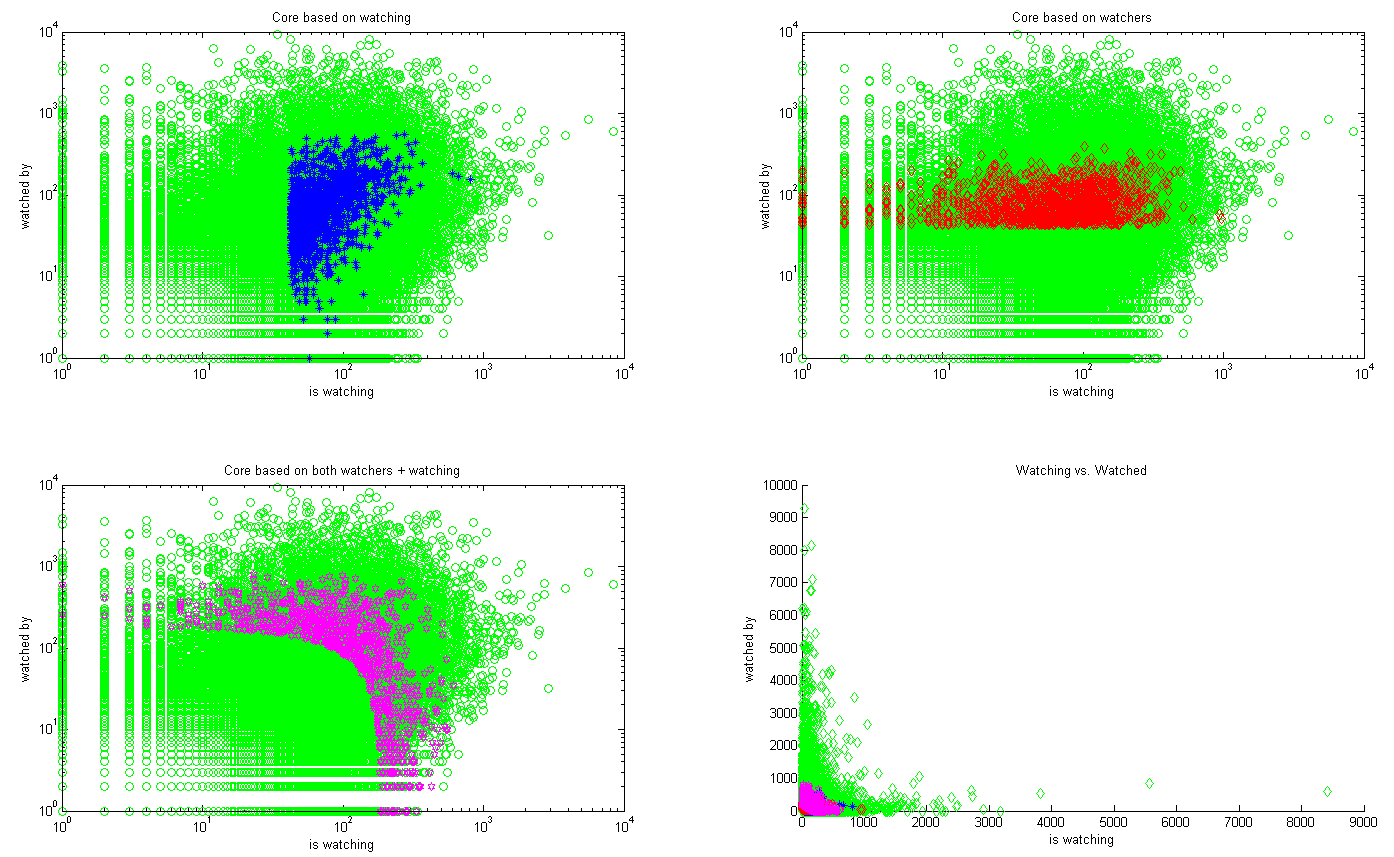
\includegraphics[width=1\linewidth]{img/core.png}
  \caption{Core networks, the degree of watching versus being watched.  The green dots represent the whole professional network, while the blue represents the watchers-core, red the watched and pink the mixed core, the last sub figure shows the power-law behavior of the degree distributions.}
  \label{fig:results_core}
\end{figure*}

Through application of the \textit{FindCore} algorithm cores of interesting artists have been identified. These cores are of manageable size for full analysis.  All core networks have a clustering coefficient larger than a comparable random network, though the mixed core is close to the random network. The characteristic path lengths are longer than their random network equivalents. This is most likely due to the relatively small size of the networks. However, the paths are still significantly smaller than $L_{lattice}=\frac{n}{2k}$. It can been concluded that the cores of dA can be considered small-world networks.  
Furthermore, the co-occurrences between the watchers and watched network is about $\frac{1}{3}$; this is much lower for the mixed network. It is presumed that this has to do with the FindCore degree $\max x$ which is much larger for the mixed network. Thus the mixed network is distinct from the watchers and watched cores which are more alike.



\subsection{Image experiments}
For the image experiments, a dataset containing full galleries of 30 artists was collected.
Those artists were selected from the \textit{daily deviations}\footnote{Daily deviations are featured images selected by dA's staff members} of a random day and includes both premium and non-premium artists. 
More details about the dataset can be found in Table \ref{datasetstats}. 
The dataset is unbalanced (like dA) since some artists only have around 50 images, while other artists have over 500 images. This may influence the performance of the classifications.



\begin{figure}[htb]
%  \centering
  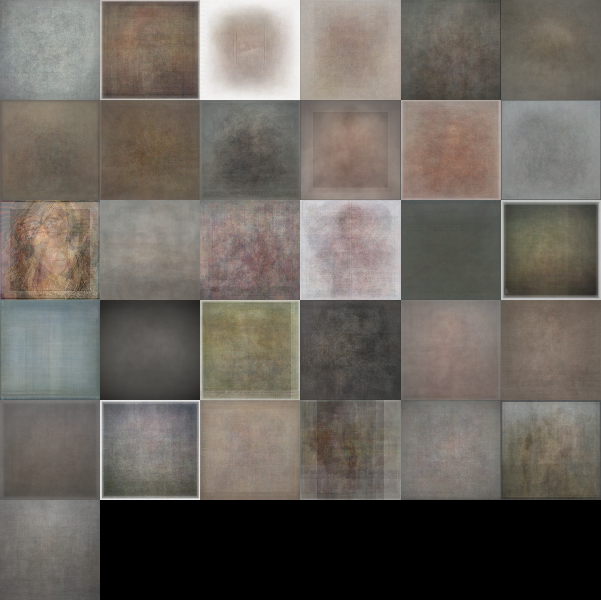
\includegraphics[width=1\linewidth]{img/datasetAvg.png}
  \caption{mean image per artist, left to right, top to bottom, in order of table \ref{datasetstats}(b): Craniata, K1lgore, Kitsunebaka91, ..., zihnisinir }
  \label{fig:avgDataset}
\end{figure}


\begin{table}[ht]
	\centering

	\subtable[General information about the dataset]{
		\begin{tabular} { |l|c| }
			\hline
			Total Size & 1.4gb \\
			\hline
			Artists & 30 \\
			\hline
			Image count & 5324 \\
			\hline 
			Average image width & 671 \\
			\hline
			Average image height & 689 \\
			\hline
			Average image size & 250kb \\
			\hline
			Average image count & 171 \\
			\hline
		\end{tabular}
	}

	\subtable [List of artist with the number of their artworks]{
		\begin{tabular}
		    { | l | c | l | c|} 
		    \hline
		    Name & count & Name & count \\
		    \hline
		Craniata &  61 & K1lgore & 63 \\
		Kitsunebaka91 & 272  & Knuxtiger4 & 193 \\
		LALAax & 82  & Mallimaakari & 151 \\
		Mentosik8 & 110 & NEDxfullMOon & 116 \\
		One-Vox & 74 & Pierrebfoto & 188 \\
		Red-Priest-Usada & 132 & Skarbog & 229 \\
		Swezzels & 9 & Udodelig & 54 \\
		UdonNodu & 38 & WarrenLouw & 51 \\
		erroid & 146 & fediaFedia & 303\\
		gsphoto & 661 & iakobos & 47 \\
		kamilsmala & 39 & miss-mosh & 307 \\
		nyctopterus & 68 & omega300m & 483 \\
		sekcyjny & 55 & stereoflow & 166 \\
		sujawoto & 33 & wirestyle & 143 \\ 
		woekan & 49 & zihnisinir & 177 \\

		    \hline 
		\end{tabular}
		\label{artists_table}
        }
	

	\subtable[Top 5 categories]{
		\begin{tabular}
		    { | l | c | } 
		    \hline
		    Category & count \\
		    \hline
		    photography & 2244 \\ 
		    customization & 906 \\ 
		    traditional & 842 \\ 
		    digitalart & 587 \\ 
		    fanart & 239 \\ 
		    \hline 
		\end{tabular}
		}
    \caption{Dataset statistics}
    \label{datasetstats}
\end{table}

Multiple experiments have been conducted in a preliminary phase, however this paper will only present results for the most significant experiment.

\subsubsection{Experimental setup}

This experiment focused on determining if an artists is distinguishable from another artist, and which are the best features to separate both. 
%This experiment is focused on finding the most defining features of every artist in the dataset.
For every artist, the feature selection algorithm uses the inter-intra criterion to select the best features.% to separate that artist from another artist.
%This is done for every artist pair in the dataset, meaning that the best 5 features can differ depending on what kind of artist pair is used.

Before performing the main experiment, another experiment was conducted to determine the performance of different classifiers.
The best performing classifier is than used for the main experiment.
The classifiers that have been used are kNN, Naive Bayes, Nearest Mean and Linear SVM.
The parameters of the classifiers have been optimized using 5-fold cross validation on 70\% of the dataset.
The remaining 30\% is used as test set for the main experiment. 
The performance measure used is $F_1$-measure.

\begin{table}[htb]
    \centering
    \begin{tabular}
        { | l | c | c |} 
        \hline
        Classifier & Mean $F_1$-measure & Stddev $F_1$-measure  \\
        \hline
        kNN & 0.7074 & 0.1731 \\ 
        Naive Bayes & 0.7897 & 0.1030 \\ 
        Nearest Mean & 0.7383 & 0.1086 \\ 
        Linear SVM & 0.8278 & 0.1450 \\ 
        \hline 
    \end{tabular}
    \caption{The mean $F_1$-measure and the standard deviation performance score of each optimized classifier on the train set using 5-fold cross-validation}
    \label{ex2optimizeresults}
\end{table}

The results are shown in Table \ref{ex2optimizeresults}.
Linear SVM has the highest mean $F_1$-measure score and the second highest standard deviation, and therefore best separates two artists.
Based on these scores, linear SVM has been selected for the main experiment.

%For this experiment each artist is compared to one other artist.
%The motivation of this approach is that each artist can be evaluated separately and it can give more clarity for cases where the performance of a classifier is low.
%The experiment is done for all the artists in the dataset meaning that an artist is compared to every other artist in the dataset.
%Also this experiment uses the feature selection algorithm to determine the features that best separates an artist from another artist.
%The feature selection algorithm selects features up to a combination of 5 different features for every artist pair.
%
%For this experiment the kNN, Naive Bayes, Nearest Mean and the SVM classifiers were optimized and trained on the train set using 5 fold cross-validation and the highest average $F_1$-measure determines the classifier that is used to produce the results.
%
%For every artist pair the $F_1$-measure is calculated on the test set to evaluate the performance of the classifier separating those artists.

\subsubsection{Image experiment results}

%Table \ref{ex2optimizeresults} shows the results After the optimization and training of the classifiers.
%The linear SVM classifier obtained the highest average $F_1$-measure however the Naive Bayes classifier did not perform significantly worse than the SVM.
%Note that the main goal of this experiment is to find feature combinations that distinguish artists.
%Therefore the focus should not go to maximizing the $F_1$-measure on the test set meaning that one classifier should be enough for this type of task.

\begin{figure*}[htb]
  \centering
  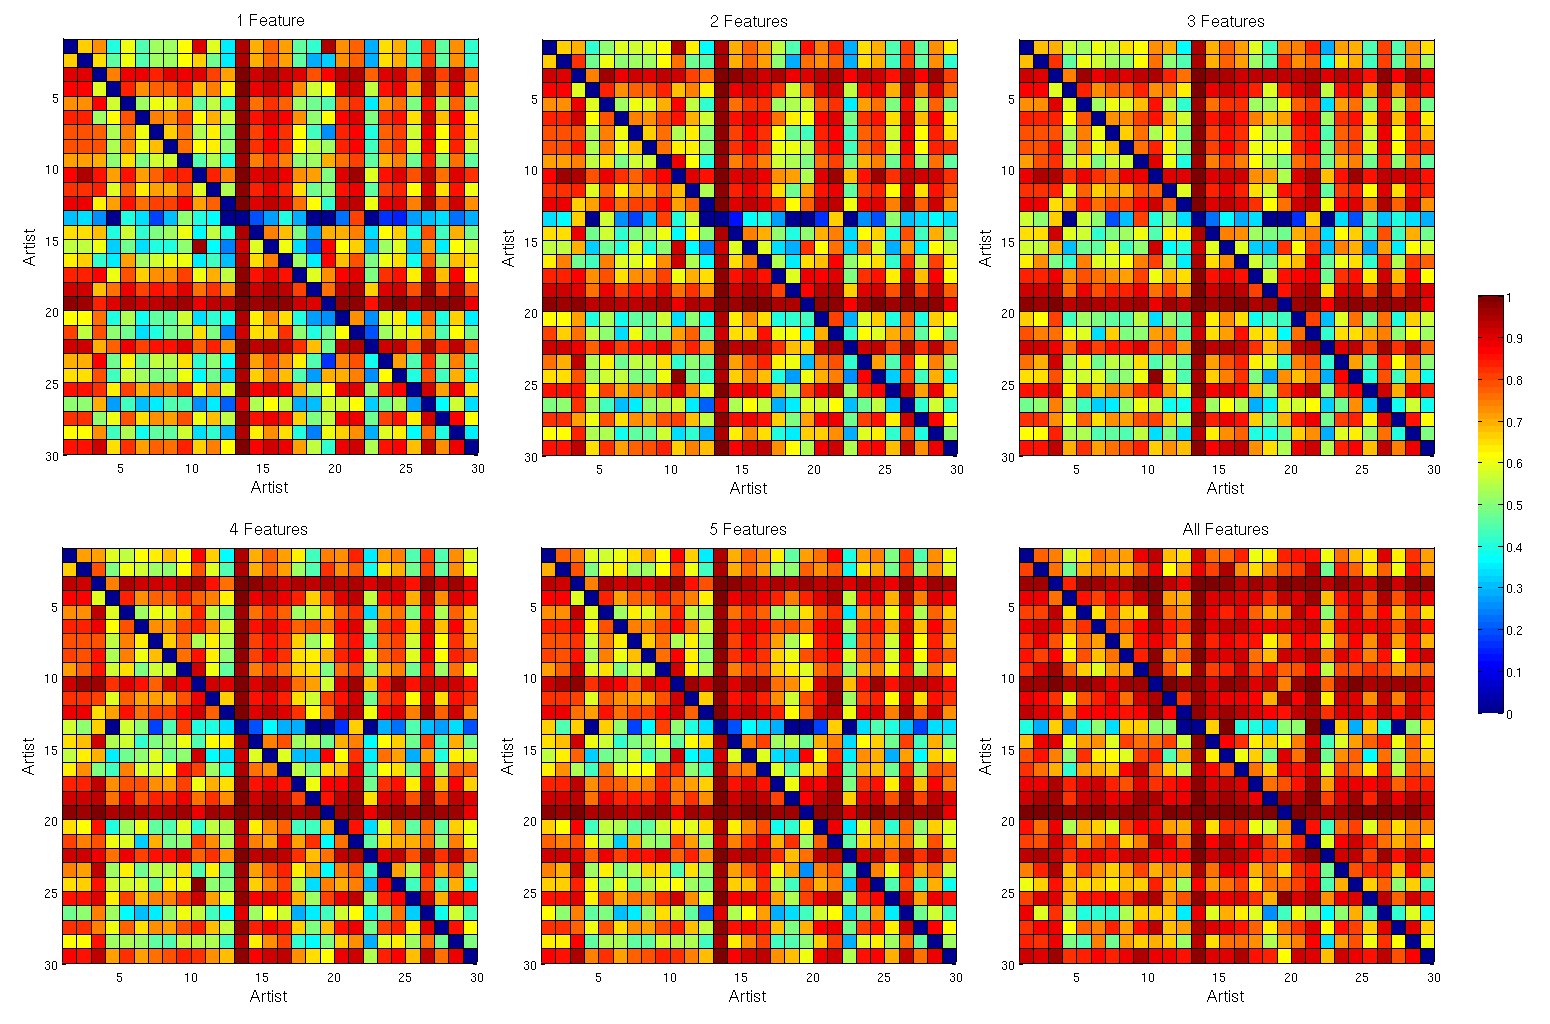
\includegraphics[width=0.75\linewidth]{img/experiment2results.png}
  \caption{The intensity mapping of the results using the linear SVM in combination with different sets of features.
  The mapping is divided into 30x30 squares where each square represents the $F_1$-measure of artist x with artist y.
  The artists are represented on both the x and the y axis by numbers.
  Table \ref{ex2stats} shows which artists are corresponding to which number.
  Also the red color represents the highest value($F_1$-measure=1).
  In the upperleft mapping, the performance using only \textit{the most} informative feature according to the selection algorithm is mapped.
  In the upperright mapping, the performance of using the \textit{3} most informative features are mapped.
  In the lowerleft mapping, the performance of using the \textit{5} most informative features are mapped.
  In the lowerright mapping, the performance of using \textit{all} the features are mapped.
  }
  \label{fig:experiment2results}
\end{figure*}

Results of the trained linear SVM on the test set are shown in Figure \ref{fig:experiment2results}.
The figure shows the \textit{intensity mappings} of four differently sized feature sets (the best 1, 3, 5 and all features).
It shows that the size of the feature sets used to separate artists is correlated to the performance score.
It also shows that there are artists pairs that can be separated using only few features.
There are artists which can be separated from all the other artists in the dataset, shown by the columns and rows that are predominantly red.
This happen because those artists use an art style that is unique in the dataset.
Furthermore, this result tells that those artists can be described using the features that are implemented in the toolkit.

\begin{table*}[htb]
    \centering
    \begin{tabular}
        { | c | l | c | c | l | } 
        \hline
        No. & Name & $\mu$ $F_1$-measure & $\sigma$ $F_1$-measure & Most defining features\\
    \hline
    1 & Craniata &  0.6314 & 0.1864 & Center average Hue, Center corner pixel ratio, Center edge to pixel ratio\\
    2 & K1lgore & 0.6078 & 0.1813 & Entropy of the Intensity, Variance of the Intensity, Edge to pixel ratio \\
    3 & Kitsunebaka91 & 0.8827 & 0.1756 & Center edge to pixel ratio, Entropy of the Intensity, Edge to pixel ratio \\
    4 & Knuxtiger4 & 0.7751 & 0.1822 & Variance of the Intensity, Entropy of the Intensity, Center edge to pixel ratio \\
    5 & LALAax & 0.6498 & 0.1902 & Edgeratio, Entropy of the Intensity, Variance of the Intensity \\
    6 & Mallimaakari & 0.7548 & 0.1824 & Variance of the Intensity, Center edge to pixel ratio, Center average Hue\\
    7 & Mentosik8 & 0.6807 & 0.1876 & Entropy of the Intensity, Variance of the Intensity, Lower-left edge to pixel ratio \\ 
    8 & NEDxfullMOon & 0.7071 & 0.1880 & Center edge to pixel ratio, Center avg B, Entropy of the Intensity\\
    9 & One-Vox & 0.6570 & 0.1833 & Entropy of the Intensity, Edge to pixel ratio, Center edge to pixel ratio  \\
    10 & Pierrebfoto & 0.8375 & 0.1852 & Entropy of the skin map, Center average Hue, Edge to pixel ratio\\
    11 & Red-Priest-Usada & 0.7376 & 0.1851 & Entropy of the intensity map, Center edge to pixel ratio, Entropy of the saliency map\\
    12 & Skarbog & 0.7875 & 0.1869 & Entropy of the Intensity, Center average saturation, Lower-right average R \\
    13 & Swezzels & 0.3296 & 0.2281 & Not enough image to report most defining features \\ 
    14 & Udodelig & 0.5798 & 0.1887 & Entropy of the Saliency, Entropy of the Intensity, $\sigma$ saliency distribution \\
    15 & UdonNodu & 0.5352 & 0.2158 & Entropy of the saliency map, Variance of the Intensity, Upper-middel average Hue \\ 
    16 & WarrenLouw & 0.6235 & 0.1864 & Entropy of the Intensity, median B, Upper-right median Intensity\\
    17 & erroid & 0.7535 & 0.1833 & Variance of the Intensity, Center edge to pixel ratio, Entropy of the Intensity\\
    18 & fediaFedia & 0.8270 & 0.1804 & Center edge to pixel ratio, Corner pixel ratio, Variance of the Intensity \\
    19 & gsphoto & 0.9172 & 0.1779 & Entropy of the Intensity, Variance of the Intensity, Center edge to pixel ratio \\
    20 & iakobos & 0.5764 & 0.1899 & edge to pixel ratio, Upper-left average saturation, upper-left median G \\
    21 & kamilsmala & 0.6359 & 0.1978 & Variance of the Intensity, Entropy of the Intensity, middle-left edge to pixel ratio\\
    22 & miss-mosh & 0.8205 & 0.1811 & upper-left corner pixel ratio, Number of faces, Entropy of the Intensity \\
    23 & nyctopterus & 0.6324 & 0.1950 & Variance of the Intensity, Center median Hue, Center average Hue\\
    24 & sekcyjny & 0.5875 & 0.1983 & Entropy of the Intensity, Lower-middle edge to pixel ratio, Entropy of the saliency map\\
    25 & stereoflow & 0.7576 & 0.1904 & Center average Hue, Variance of the Intensity, Corner pixel ratio \\
    26 & sujawoto & 0.4752 & 0.1873 & Entropy of the intensity map, Entropy of the Intensity, Lower-middle edge to pixel ratio\\
    27 & wirestyle & 0.7138 & 0.1931 & Entropy of the intensity map, Variance of the Intensity, Center average B\\ 
    28 & woekan & 0.5529 & 0.1881 & Entropy of the Intensity, Variance of the Intensity, Upper-left edge to pixel ratio\\
    29 & zihnisinir & 0.7632 & 0.1918 & Entropy of the Intensity, Center average saturation, Entropy of the intensity map\\
    30 & omega300m & 0.8318 & 0.2403 & Entropy of the Intensity, Center edge to pixel ratio, Lower-right average Intensity \\
        \hline 
    \end{tabular}
    \caption{This table first describes the mean $F_1$-measure and its standard deviation for every artist which was computed by using linear SVM combined with a feature set containing the 5 most informative features that separates an artist pair.
    It also shows the number of the artist that corresponds to the x/y axis of the intensity mappings found in figure \ref{fig:experiment2results}.
    The last column shows the most defining features that can describe the artist.}
    \label{ex2stats}
\end{table*}

Table \ref{ex2stats} shows the most discriminating features for each artist. 
Based on these results, some observations can be made.
For some artists the mean $F_1$-measure is very low. This shows that despite the features are the best ones in the entire feature collection, they are not sufficiently describing the artists.
The table shows that the \textit{edge to pixel ratio} and \textit{intensity} are valuable features in describing artists.
This is very feasible because images can range between being dark and very light. Moreover, there are styles that have many edges (e.g. photographs and drawings), but more abstract ones that have not.
Other discriminant features are \textit{hue} and \textit{corner pixel ratio}.
Even more, it seems that cognitive-inspired features perform best on certain styles.
For example, the artist $Pierrebfoto$ has a lot of nude images and this was exploited by the skin map feature.
Another important detail about these results is that the center cell of an image is chosen a lot compared to the other cells.
This is actually highly feasible because most of the time in an image, the center contains the most information.